\section{Změna světlosti a kontrastu}
Prvním úkolem po konzultaci se školitelem bylo pokud je to možné odstranění knihovny Cg toolkit z kódu programu \cite[str. 23]{flaska}. Při prvních pokusech o nasazení programu do zkušebního provozu v IKEM dělala tato knihovna velké potíže. Program nefungoval na počítačích s grafickou kartou NVIDIA GeForce, respektive fungoval, ale bez stěžejní součásti pro změnu světlosti  kontrastu zobrazovaných snímků. Tyto funkce jsou však velice důležité (dle lékařů z IKEM), protože výrazně ovlivňují to, co bude na snímku vidět.

Dalším důvodem pro odstranění závislosti na knihovně Cg Toolkit je to, že program závisí již na více než pěti externích knihovnách a to komplikuje překlad. Více viz~\pageref{sec:preklad} 

Pro odstranění závislosti na knihovně Cg toolkit je potřeba pochopit, co přesně kód této části programu provádí, a dále dohledat vhodné řešení problému bez použití knihovny Cg toolkit, tj. s použitím pouze OpenGL. Bc. Neškudla obhajuje ve své práci použití Pixel Shaderu tím, že při stejných transformacích prováděných pomocí OpenGL dojde ke ztrátě dat obrazu. Tato kapitola vysvětlí, co znamená změna světlosti, respektive kontrastu snímku, proč dochází ke ztrátě dat a jak tyto tranfsormace provádět aby ke ztrátě dat nedošlo.

\subsection{Světlost a kontrast}
Pro naprogramování funkcí pro změnu světlosti a kontrastu je potřeba nejprve pochopit o jaké matematické operace se jedná. V našem případě se můžeme omezit jen na černobílé snímky, protože výstupem MRI jsou pouze černobílé snímmky. Obrázek tedy můžeme chápat jako matici čísel mezi $0$ a $1$, kde sloupce, respektive řádky odpovídají souřadnicím bodu v obrázku:

\[
 Im_{res_{x},res_{y}} =
 \begin{pmatrix}
  Im(1,1) & Im(1,2) & \cdots & Im(1,res_{x}) \\
  Im(2,1) & Im(2,2) & \cdots & Im(2,res_{x}) \\
  \vdots  & \vdots  & \ddots & \vdots  \\
  Im(res_{y},1) & Im(res_{y},2) & \cdots & Im(res_{y},res_{x})
 \end{pmatrix}
\]

kde \[ Im(x,y) \in [0,1] \]

Pro $ Im(x,y) = 0 $ vidíme pixel naprosto černý, pro $ Im(x,y) = 1 $ vidíme pixel bílý.

Světlost je pak slovně definována jako množství světla jež vyzařuje zdroj. Matematicky přesnější definice pak je:

\emph{Světlost je definována jako střední hodnota světlosti všech bodů.}

Matematicky zapsáno:
\[
  Brightness(Im) = \frac{1}{res_{x}*res_{y}}\sum_{\substack{0 \leq x \leq res_{x} \\ 0 \leq y \leq res_{y}}} Im(x,y)
\]
Změnou světlosti snímku je pak zvětšení, či zmenšení uvedené střední hodnoty. Zpravidla se světlost mění přičtením konstanty ke světlosti všech bodů. Tj. pro bod o souřadnicích $x,y$.
\[
Im(x,y) \longmapsto Im(x,y) + c_{brightness}
\]

Situace s kontrastem snímku je mírně komplikovanější. Kontrast je pro černobílý snímek slovně definován jako rozdíl ve světlosti tmavých a světlých bodů. Tuto vlastnost vystihují nejméně dvě různé definice kontrastu:

Michelsonův kontrast:

\[
Contrast(Im) = \frac{Im_{max}-Im_{min}}{Im_{max}+Im_{min}}
\]

kde:
\[
Im_{max} = \max_{\substack{ 0 \leq x \leq res_{x} \\ 0 \leq y \leq res_{y} }}{Im_{x,y}} 
\]
\[
Im_{min} = \min_{\substack{ 0 \leq x \leq res_{x} \\ 0 \leq y \leq res_{y} }}{Im_{x,y}}
\]

jedná se o jednodušší a názornější definici kontrastu, bohužel však v některých případech neodpovídá pozorovatelným vlastnostem. Takto počítaný kontrast totiž není robustní vůči výchylkám jednotlivých bodů. Představme si snímek $1000*1000$ bodů, kde světlost téměř všech bodů se bude pohybovat mezi hodnotami $0.4$ a $0.6$, světlost jednoho bodu bude $0$ a světlost dalšího bodu bude $1$. V tomto případě je kontrast snímku $1$. Po přeškálování světlosti uvedených dvou bodů na hodnotu $0,5$ se rázem změní kontrast snímku na hodnotu $0,2$. Přitom jsme během změny kontrastu na snímku nemohli pozorovat prakticky nic.

Vhodnější definice kontrastu by tedy byla následující:

Root Mean Square Contrast:
\[
Contrast(Im) = \sqrt{\frac{1}{res_{x}*res_{y}}\sum_{\substack{ 0 \leq x \leq res_{x} \\ 0 \leq y \leq res_{y} }}(Im_{x,y}-Brightness(Im))^2}
\]

Vzorec pro výpočet kontrastu nápadně připomíná výpočet rozptylu náhodné veličiny. 

Při porovnání obou vzorců vidíme, že první vzorec je velice jednoduchý na výpočet, ale výsledek přesně nevystihuje vizuální dojem z obrázku. Druhý výpočet je výrazně náročnější na výpočet, ale je také nesrovnatelně přesnější. Jako vhodná alternativa se tak nabízí používat druhý vzorec, ale do sumy dosadit pouze náhodný výběr bodů z obrázku.

Změna kontrastu snímku se ve většině počítačových programů provádí podle následujícího pravidla pro světlost bodu:
\[
  Im(x,y) \longmapsto   (Im(x,y) - 0.5)*c_{contrast} + 0.5
\]

Původní hodnotu svělosti pixelu zmenšíme o $0.5$. Díky tomuto kroku pak při násobení získané hodnoty koeficientem $c_{contrast}$ docílíme toho, že pixely s původní světlostí pod $0.5$ získají ještě nižší hodnotu světlosti, naopak pixely se světlostí nad $0.5$ získají vyšší světlost. Dále přičteme hodnotu $0.5$ a tím se vrátí hodnoty světlosti na původní úroveň.

Nejlépe je pak vidět uvedená transfmormace, když si její transformační křivku. Na transformaci $ Cont(*,c_{contrast}) $ se můžeme dívat jako na funkci jedné proměnné na intervalu $[0,1]$. Pro vstupní hodnotu $ Im(x,y) $ získáme výstupní hodnotu $ (Im(x,y) - 0.5)*c_{contrast} + 0.5 $.

Pro $ c_{contrast}=1 $, tedy pro transformaci, jež zachová obrázek v původním stavu, bude graf funkce $ Cont(*,c_{contrast}) $ vypadat následovně:

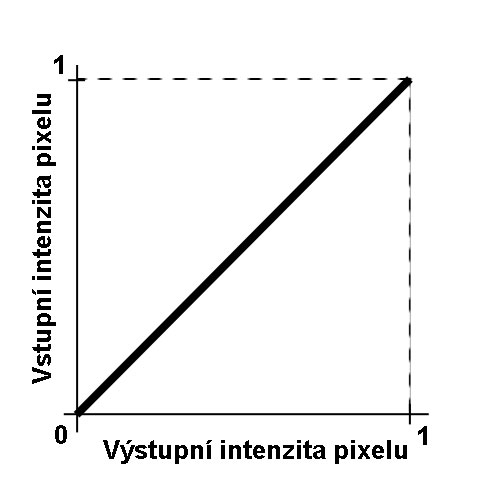
\includegraphics[width=0.7\textwidth,height=0.7\textwidth]{Text/IMG/Kontrast_Identita.jpg}

Pixel o vstupní intenzitě $0.25$ bude mít výstupní intenzitu $0.25$.

Ukažme si nyní, jak vypadá stejná křivka pro transformaci, která kontrast obrázku zvyšuje, např. pro $ c_{contrast}=1.25 $.
Vezmeme-li v úvahu uvedený vzorec a vezmeme-li dále v úvahu podmínku $ Im(x,y) \in [0,1] $.

Pak můžeme křivku transformace pro $ c_{contrast}=1.25 $ načrtnout takto:

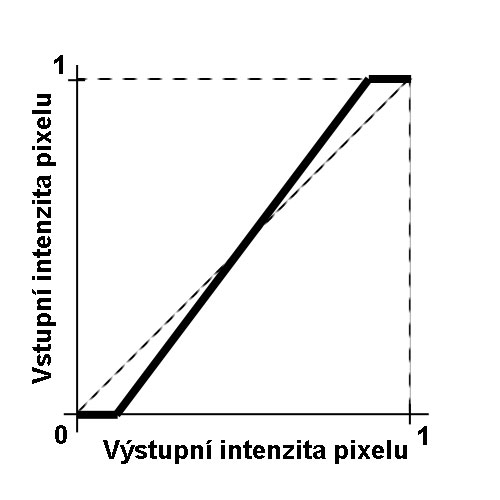
\includegraphics[width=0.7\textwidth,height=0.7\textwidth]{Text/IMG/Kontrast_Transformace_1.jpg}

Křivka na obrázku má strmější spád. To znamená, že světlejší pixely (s původní světlostí $> 0.5$) se staly ještě světlejší a naopak tmavší pixely (s původní světlostí $< 0.5$) ještě více ztmavly. Z uvedeného nákresu je pak vidět co vyplývá z předpisu transformace a podmínek $ Im(x,y) \in [0,1]$. Při zvýšení kontrastu koeficientem k se intenzita všech bodů, jejichž intenzita je z intervalu $ [0,\frac{1}{2k}] $, změní na $0$ a dále intenzita všech bodů, jejíchž původní intenzita byla v intervalu $[1-\frac{1}{2k},1]$, se změní na hodnotu $1$. Jinými slovy, jak se v odborné terminologii užívá, dojde ke ztrátě grafické informace a to v uvedených množinách bodů. Volnější parafrázi bychom řekli, že odstíny největlejší bodů se slijí do jediného odstínu a odstíny nejtmavších bodů se slijí do jediného odstínu, více na následujícím příkladu:

\begin{table}%[ht]
	\caption{Příklad příliš výrazné změny kontrastu, kdy dochází ke ztrátě grafické informace.}
		\begin{tabular}{p{7cm}p{7cm}}
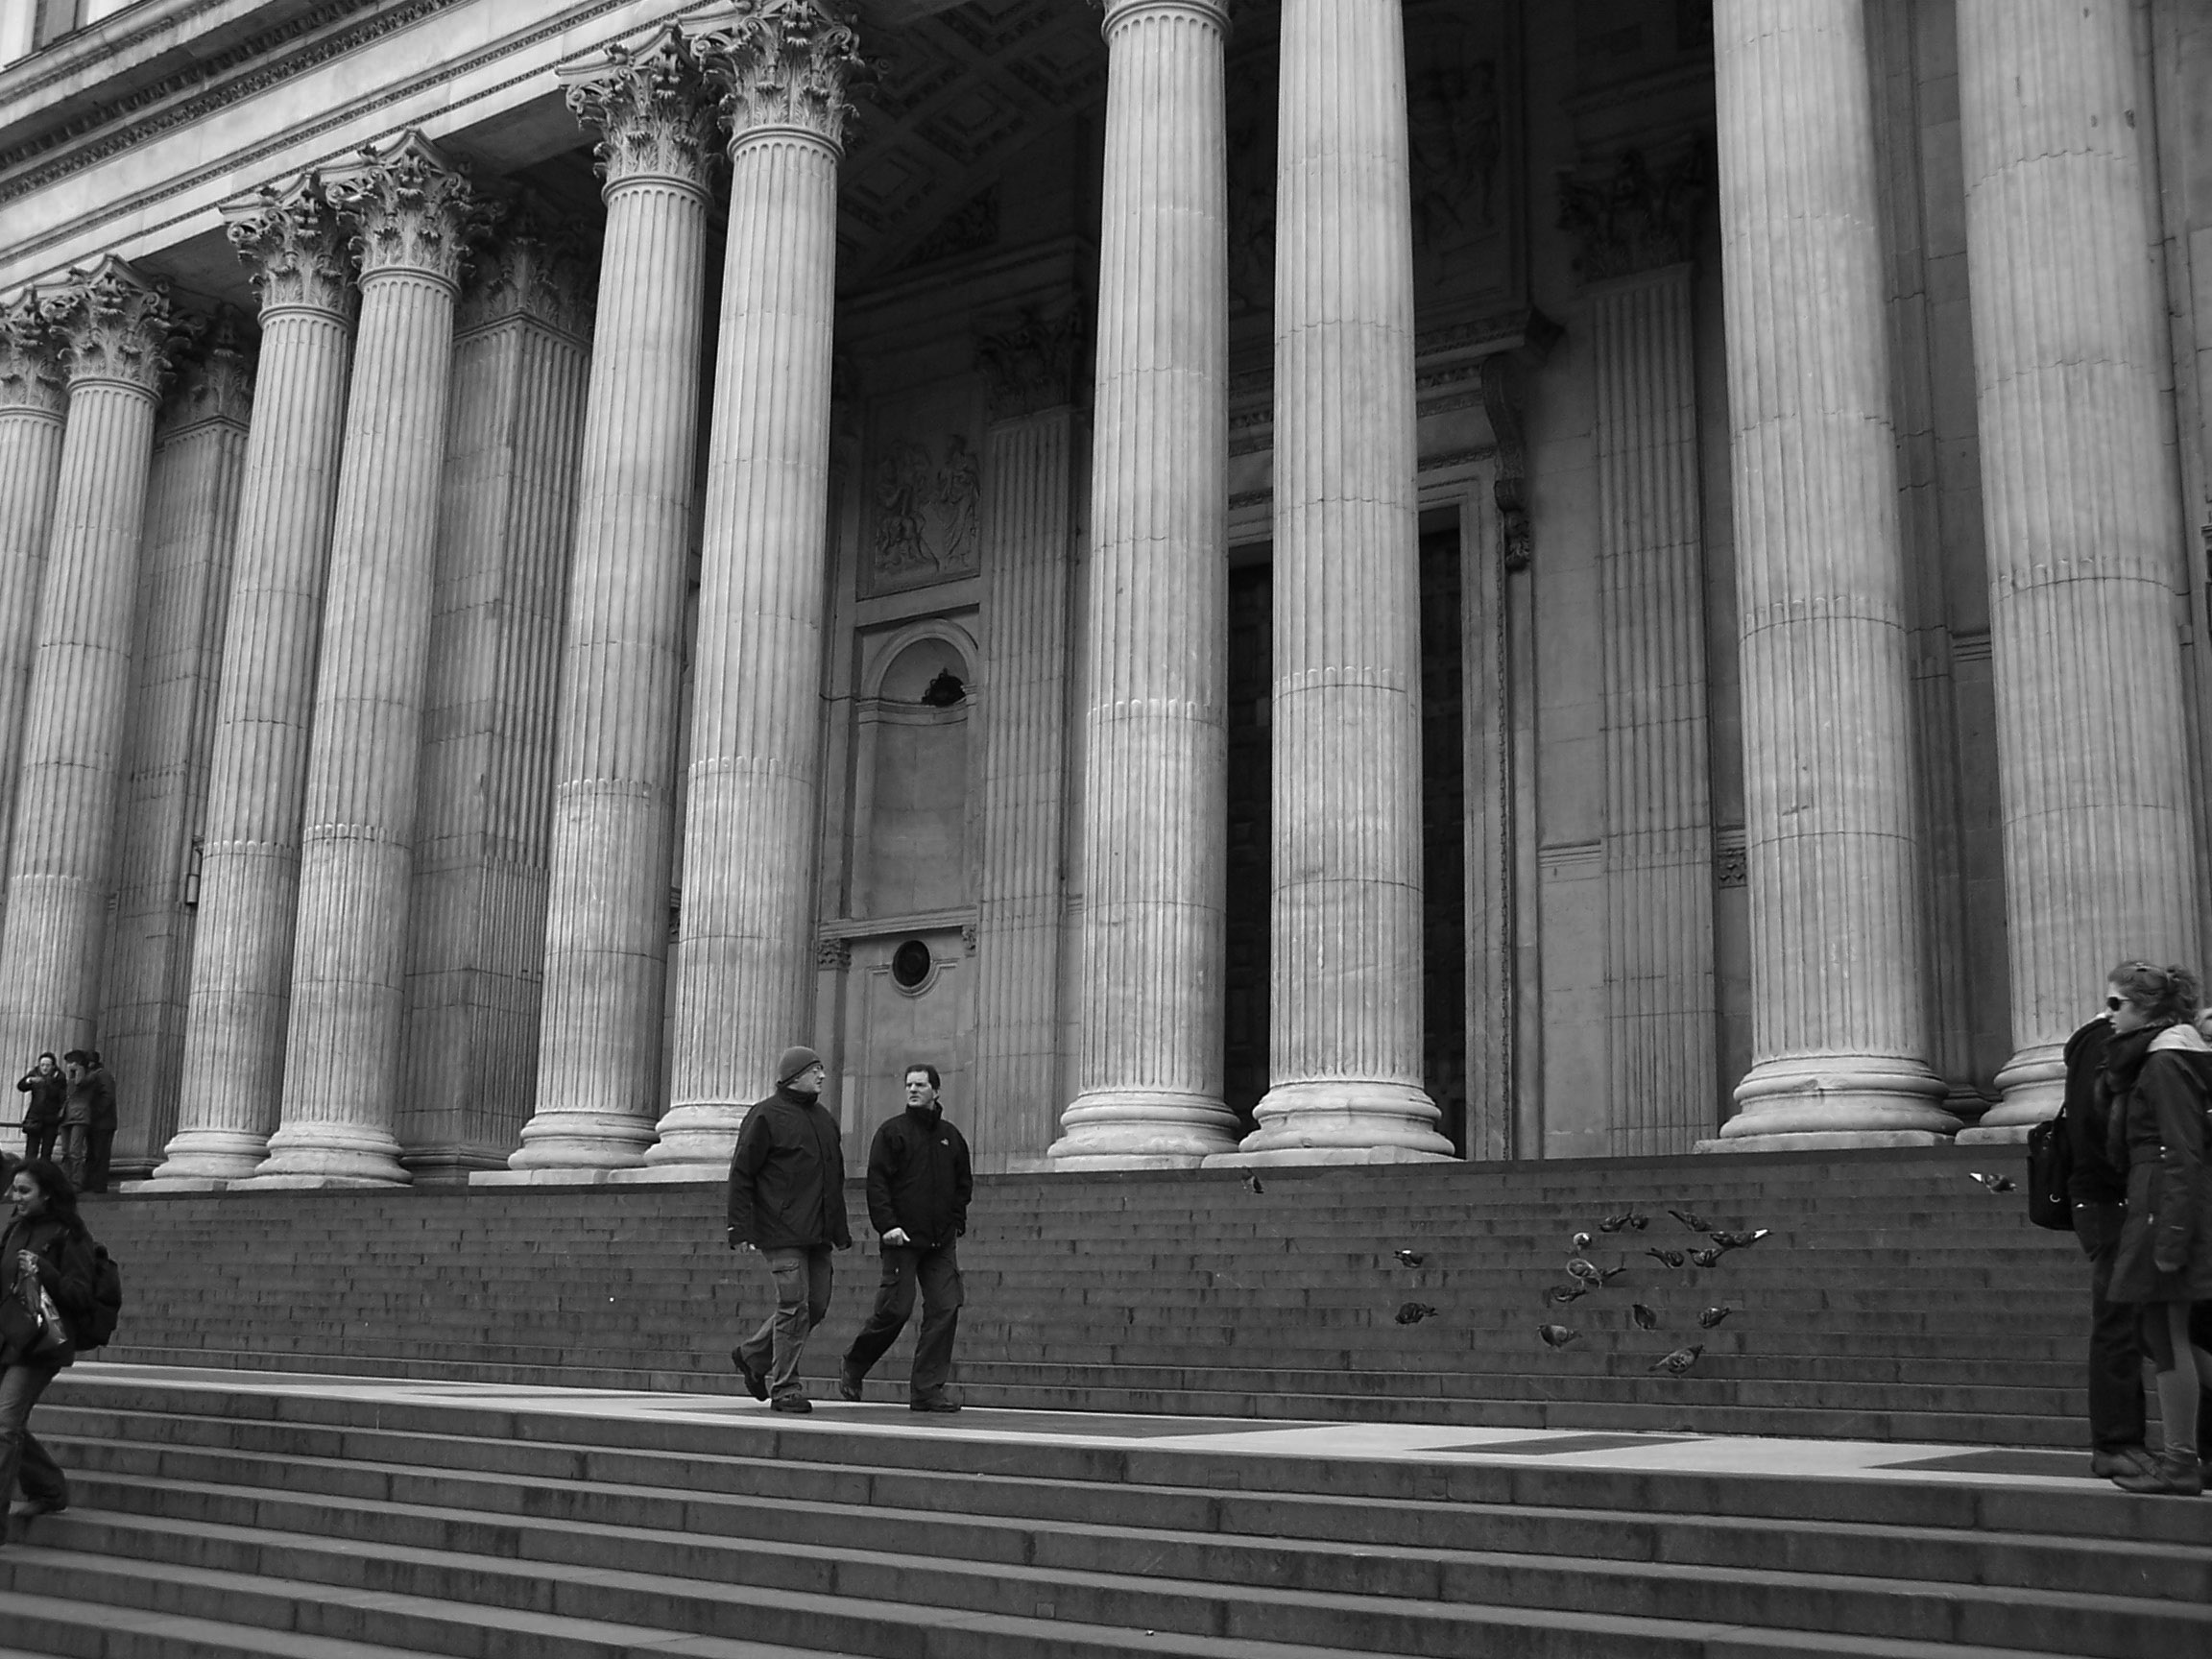
\includegraphics[width=0.5\textwidth,height=0.35\textwidth]{Text/IMG/London.jpg} & 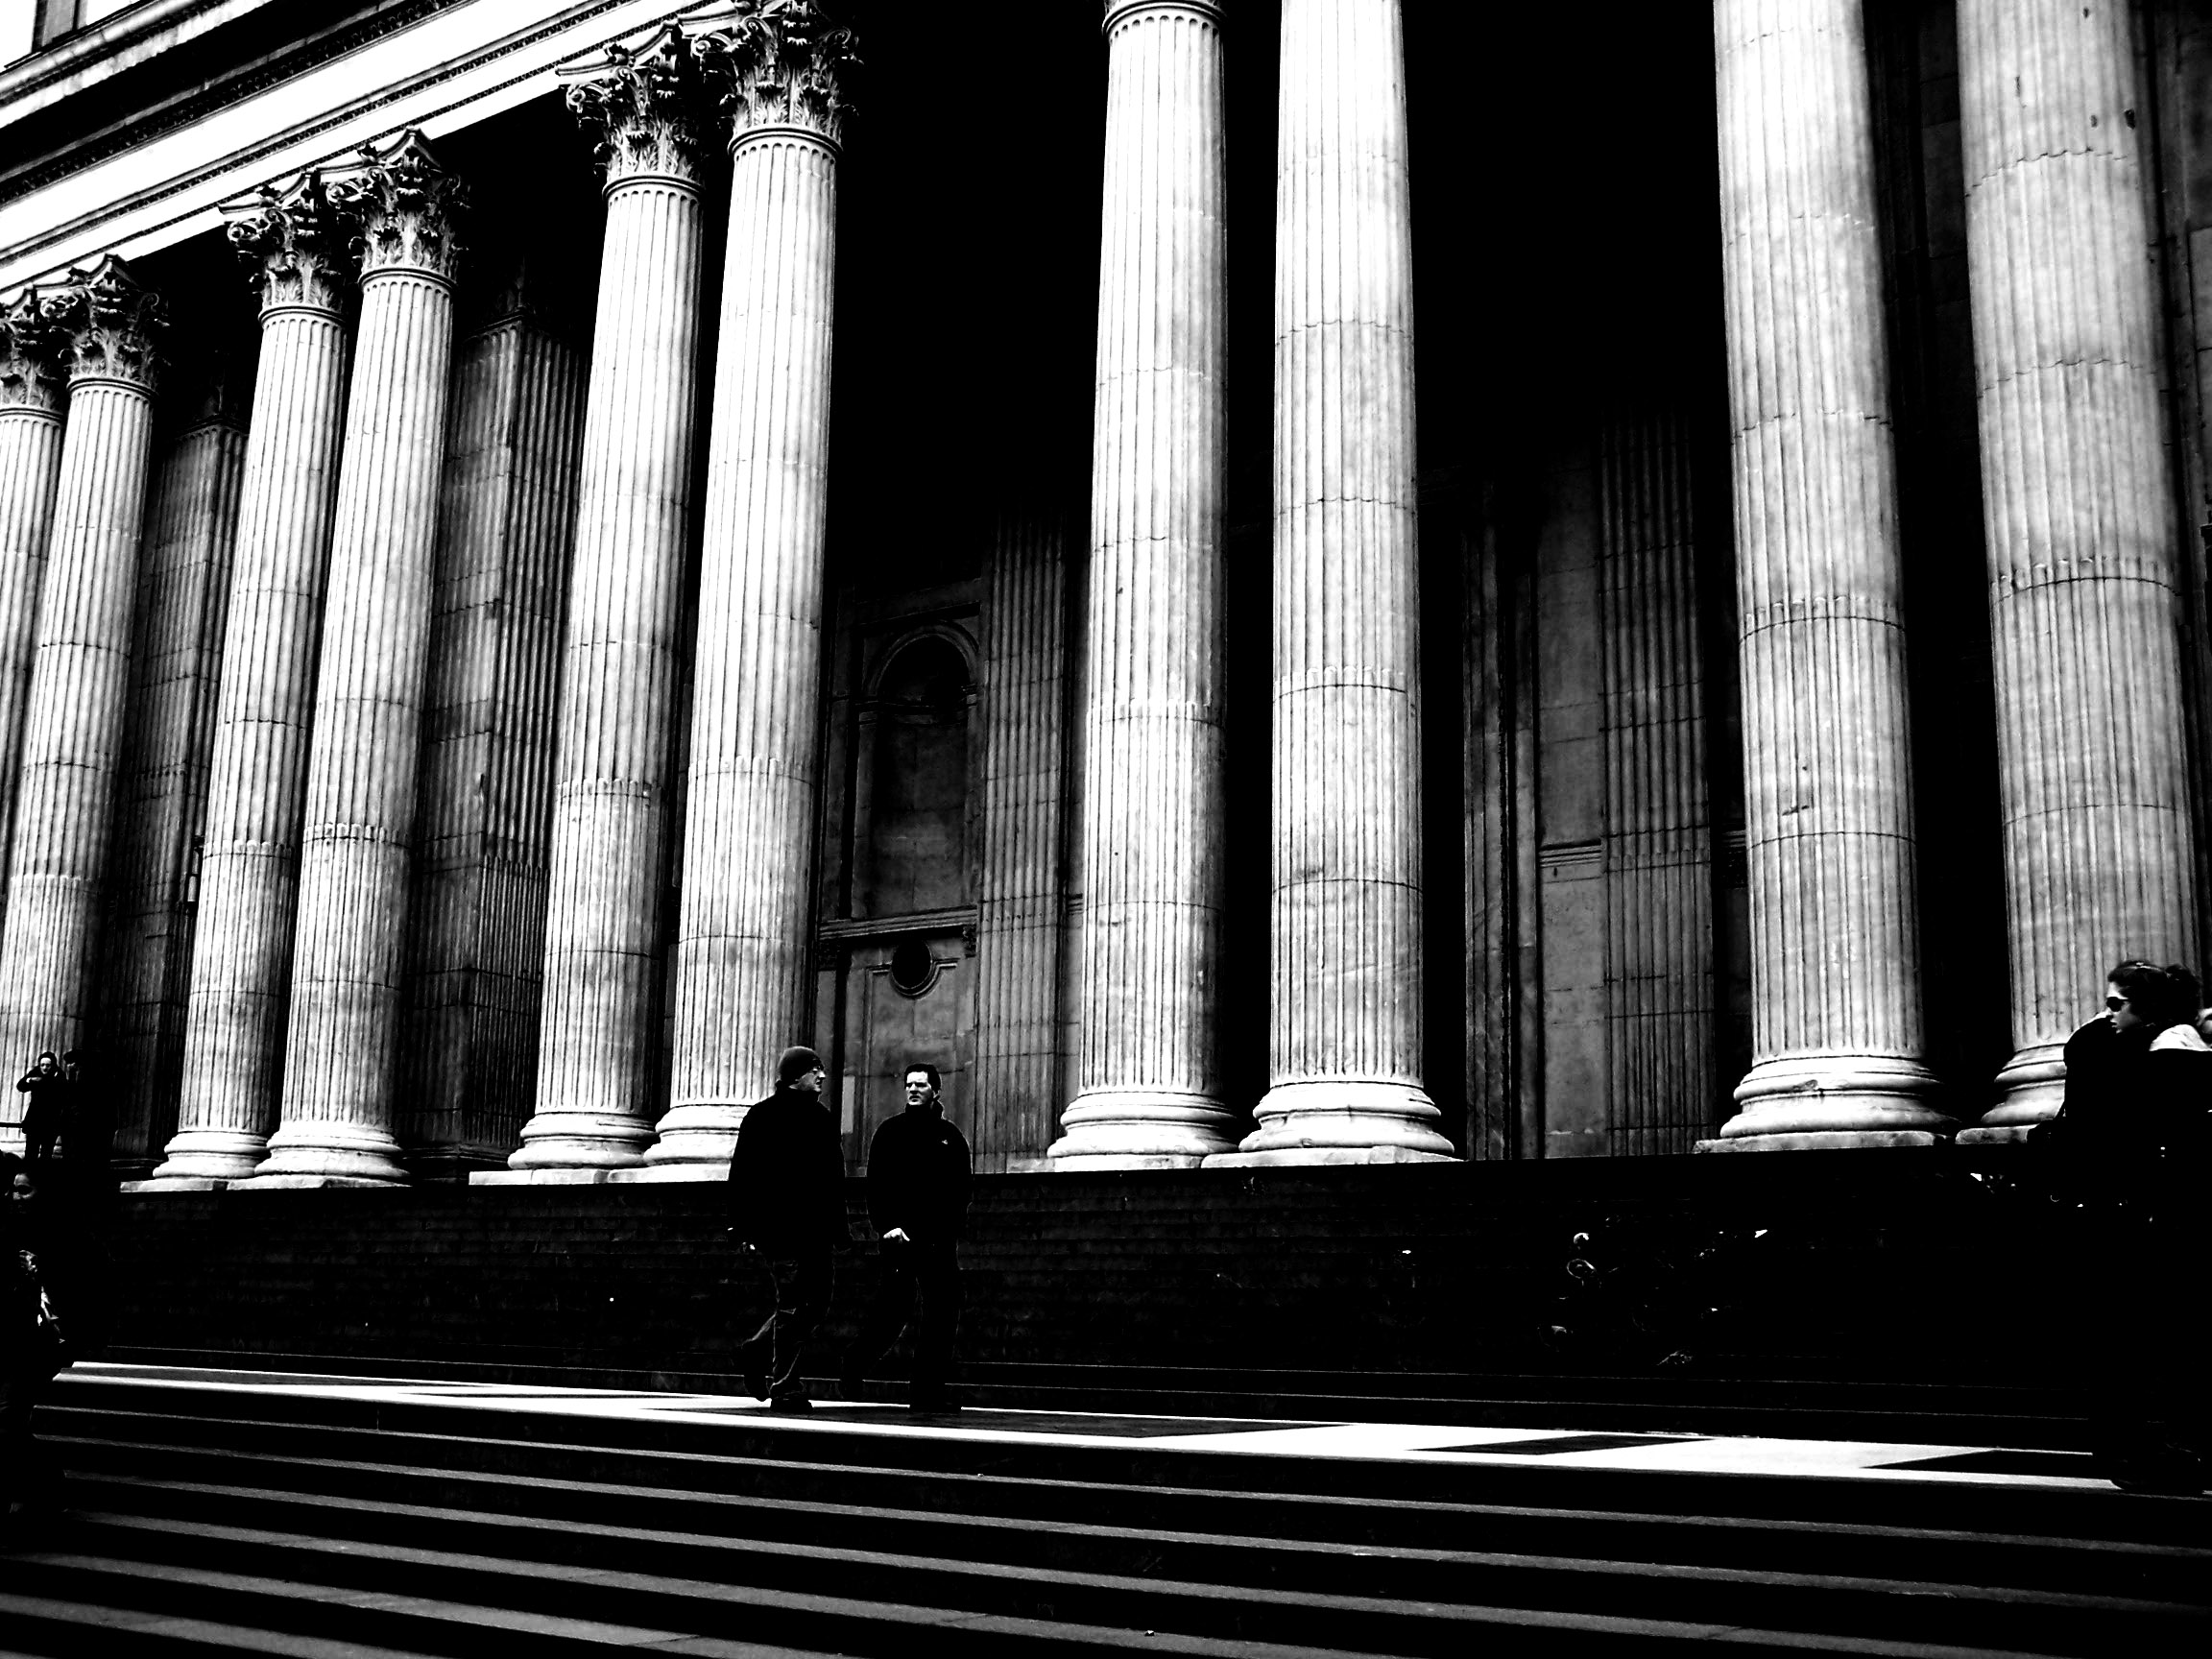
\includegraphics[width=0.5\textwidth,height=0.35\textwidth]{Text/IMG/London_High_Contrast.jpg} \\
\center{Původní obrázek.} & \center{Obrázek po změně kontrastu.}\\
		\end{tabular}
\end{table}

Nejmodernější počítačové programy pak používají nelineární transformace pro změnu kontrastu. Při jejich použití nedochází ke ztrátě grafické informace. Křivka takové transformace pak vypadá přibližně takto: 

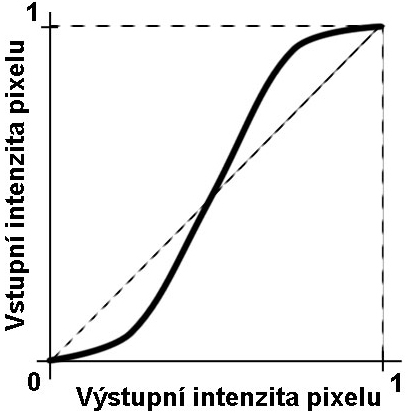
\includegraphics[width=0.7\textwidth,height=0.7\textwidth]{Text/IMG/Kontrast_Transformace_2.jpg}

